\section{Agricultural Platooning Services}

After I analyzed the impact on data rate and robustness of the physical layer parameters, I will simulate a platooning scenario in ns-3 to find the influence of the physical layer configuration on the network performance.


The network performance metric consists of the latency, which describes the time needed to transmit the data
on the application layer, and the update rate of the platooning service, which defines how long ago a new position update
was received by the \ac{TM} in the Platooning Service.

Ns-3 is suitable for this simulation because it supports application layer-level simulation.
Via the extension Netsimulyzer, a graphical user interface is available to visualize the simulation results.

Any packets in ns-3 can be tagged with a ns-3 Packet Tag \footnote{\url{https://www.nsnam.org/docs/release/3.36/doxygen/classns3_1_1_tag.html}},
which are designed to add additional information to the packet.
Every added ns-3 Packet Tag belongs to the packet and does not change the packet size or characteristics.
Throughout the simulation, I used ns-3 Packet Tags to add information that needed transferring.

The simulation scenario is based on the corn harvest and loading scenario, which is described in \autoref{sec:corn_harvest_scenario}, where
multiple \ac{FH}s harvest the corn and load it onto one of the \ac{TM}s.

An ns-3 Node represents every machine.
Each Node has a mobility model, which describes the movement of the machine.

\subsubsection*{Wi-Fi Setup}
In order to exchange data between the machines, every machine is equipped with an  ns-3 IEEE 802.11ax WifiNetDevice.
Every Wi-Fi Device runs in Ad-Hoc mode to enable direct communication
between the machines.
The Wi-Fi data rate is managed by a Constant Rate Wi-Fi Manager, which has a non-uniform
transmission mode and a data mode for uniform transmissions.
The transmission modes are configured according
to the parameters in \autoref{tab:SimulationParametersWiFi}.

The parameters are chosen from the results of the physical layer analysis of \autoref{sec:DataRate} and \autoref{sec:Robustness}.
Non-uniform transmissions are used to broadcast the Agricultural Platooning Service advertisements.

The non-uniform transmission parameters enable the longest possible
transmission range, which results in the lowest data rate.
Since no high data rate is required to advertise the Service, I chose the parameters to maximize the transmission range.
As aforementioned, ns-3 does not support \ac{DCM} at the moment.
In order to implement \ac{DCM} in the simulation, I doubled the data length for \ac{DCM} enabled transmissions to
represent the overhead of transmitting redundant copies of data for \ac{DCM}. \ac{DCM} would utilize the copies to determine the
correct data via maximum likelihood decoding.
As a result, the communication would be more robust, as shown in \autoref{sec:Robustness}.
This effect is not included in the current version of the simulation.

Guidance data in the Agricultural Platooning Service is exchanged between the \ac{FH} and the \ac{TM} via the
uniform transmission mode.
The process data in \autoref{chap:cornHarvestData} reflects that a short transmission range
is sufficient to exchange the guidance data, which must still be robust against multipath effects.
I chose the parameters to balance a high robustness and high data rate.
The uniform transmission parameters are changed in the simulation to analyze the impact on the network performance metrics.

Similar the ns-3 simulation in \autoref{sec:DataRate}, this simulation is based on the ns-3 ConstantSpeedPropagationDelayModel, the ns-3 FriisPropagationLossModel and
the ns-3 TableBasedErrorRateModel.

\begin{table}[H]
   \centering
   \begin{tabular}{p{6cm}p{4cm}}
      General Parameters & \\
      \midrule
      Wi-Fi Standard & IEEE 802.11ax\\
      \ac{GI} & \SI{3200}{\nano\second}\\
      \ac{LDPC} enabled & True\\
      Frequency Spectrum & \SI{5.6}{\giga\hertz}\\
      \ac{BW} & \SI{20}{\mega\hertz}\\
      Max. Transmission Power & \SI{25}{\decibel}\\
      Antenna Gain & \SI{5}{\dB}\\
      Maximum retries & \num{3}\\
       & \\
      Uniform Transmission Parameters & \\
      \midrule
      \ac{MCS} & \num{5}\\
      Number \ac{MIMO} Streams & \num{2}\\
       & \\
      Non-Uniform Transmission Parameters & \\
      \midrule
      Broadcast \ac{MCS} & \num{0}\\
      \ac{ER} mode enabled & True\\
      \ac{DCM} enabled & True\\
   \end{tabular}
   \caption{Default simulation parameters for Wi-Fi Devices on \acf{FH} and \acf{TM}}
   \label{tab:SimulationParametersWiFi}
\end{table}

\subsubsection*{Agricultural Platooning Service}
Every machine node runs an ns-3 Application responsible for the Agricultural Platooning Service.
The application is identified by a unique identifier and runs a \ac{UDP} socket to exchange data with other Agricultural Platooning Service applications.
Every \ac{UDP} socket can be addressed by an IP address and a port number.
The IP address is the IP address of the machine node.

Every \ac{FH} starts in the lower left corner of the field and harvests the corn along the path,
which is displayed in \autoref{fig:PlatooningRoute}.
As soon as a \ac{FH} reaches a field border, it makes a U-turn and continues
in the opposite direction.
Every \ac{FH} harvests the corn until it reaches the end of the field in the lower right corner.
The initial position of the \ac{TM}s is a row below the \ac{FH}s, which is displayed in \autoref{fig:PlatooningInit}.
\begin{figure}[H]%
   \centering
   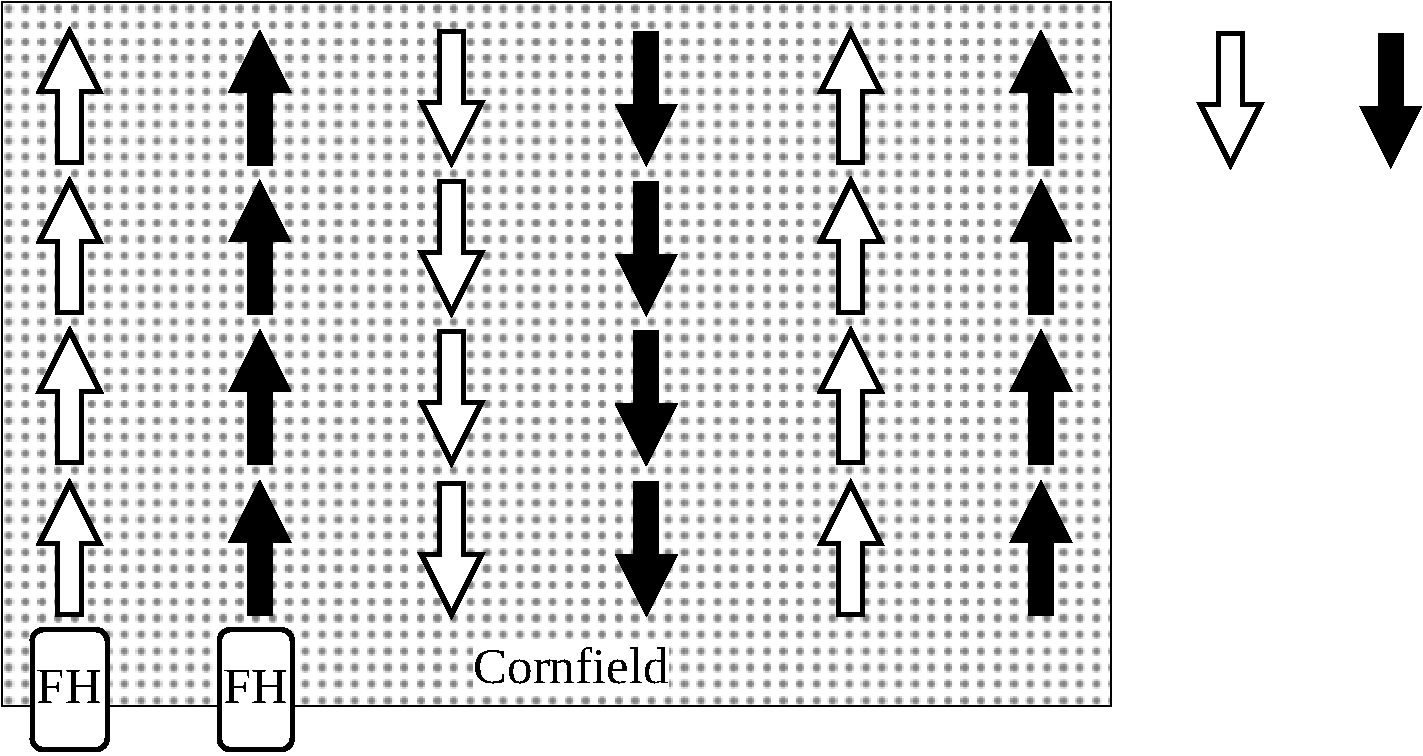
\includegraphics[width=0.7\textwidth]{figures/drawings-Route}
   \caption{Path of the \acf{FH} for harvesting corn on the field}
   \label{fig:PlatooningRoute}%
\end{figure}

In the beginning, every \ac{FH} broadcasts a search request $search\_TM$ via the non-uniform transmission mode to find an empty \ac{TM} to load the corn onto according to
to the procedure in \autoref{alg:SearchTM}.
As shown in \autoref{fig:PlatooningInit}, multiple \ac{TM}s receive the search request and answer with
their current fill level of the \ac{TM}'s trailer.
The \ac{FH} chooses the \ac{TM} with the lowest fill level and sends a connection request to the \ac{TM}.
As soon as the \ac{TM} receives the connection request, it answers with a connection response.
When the \ac{FH} receives the connection response, the Agricultural Platooning Service is started.
When no \ac{TM} answers the search request, the \ac{FH} repeats the search request every $search\_TM\_interval$ seconds.

\begin{figure}[H]%
   \centering
   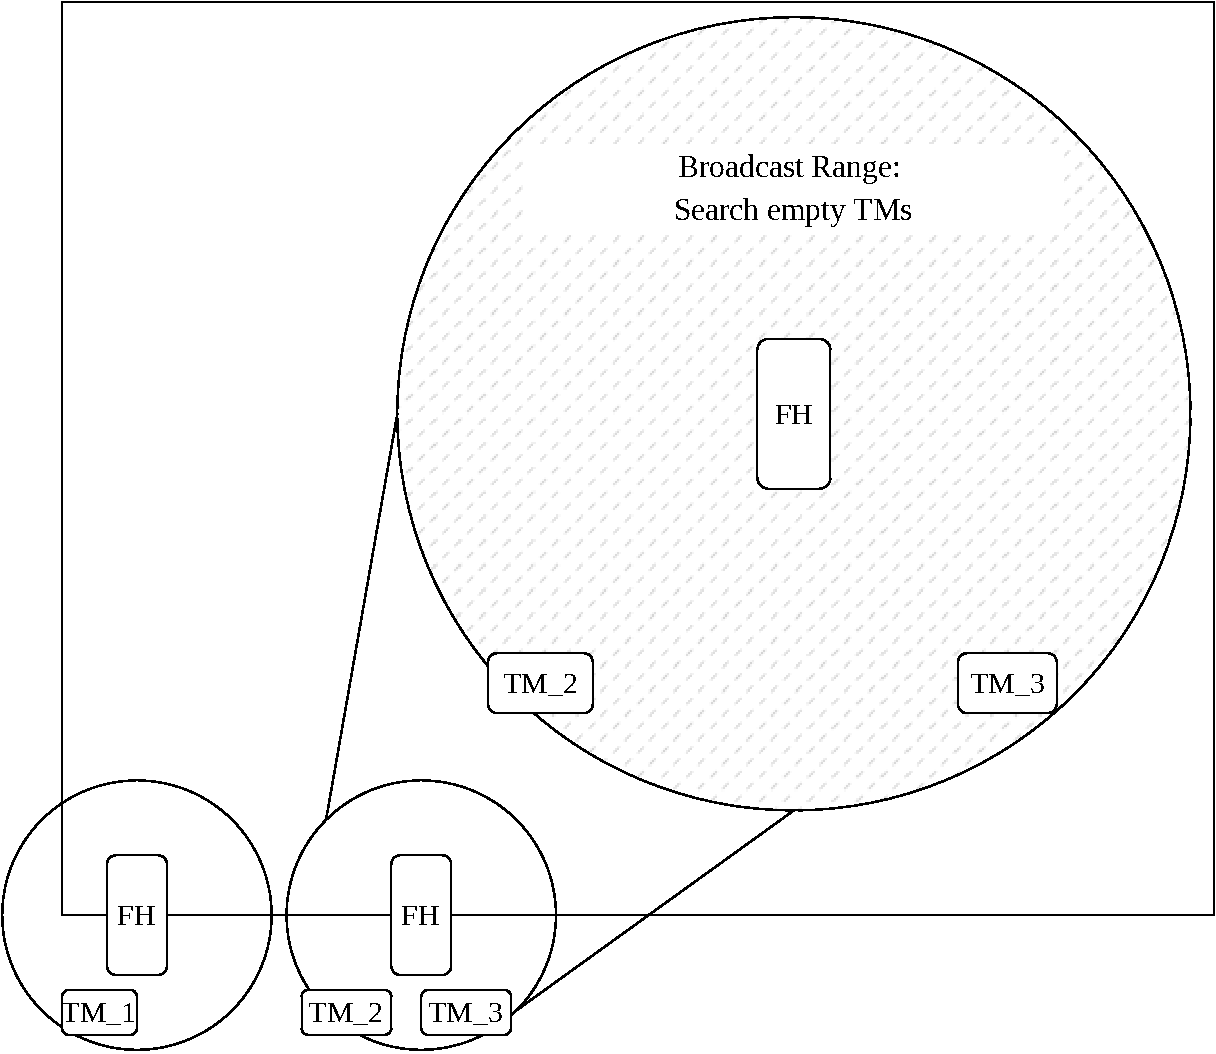
\includegraphics[width=0.7\textwidth]{figures/platoonINIT}
   \caption{Start position of the \acf{FH}s and \acf{TM}s, where a \ac{FH} broadcasts a search request to find
   a \ac{TM} to load the corn onto}
   \label{fig:PlatooningInit}%
\end{figure}

\begin{algorithm}
\begin{algorithmic}[1]
\REQUIRE Defined $search\_TM\_interval$, $search\_TM\_packet\_length$
\STATE Create packet $search\_TM$ of length $search\_TM\_packet\_length$ bytes
\STATE Broadcast $search\_TM$ to all \acs{TM}s
\IF {no \acs{TM} ansers}
    \STATE Repeat Broadcasting $search\_TM$ every $search\_TM\_interval$ seconds
\ELSE
   \STATE Send connection request
   \IF {No \acs{TM} response}
      \STATE Repeat Broadcasting $search\_TM$ every $search\_TM\_interval$ seconds
   \ELSE
      \STATE Connection established
      \STATE Start Agricultural Platooning Service
   \ENDIF
\ENDIF
\end{algorithmic}
\caption{Procedure of the \acf{FH} to search for a \acf{TM} to load the corn onto}
\label{alg:SearchTM}
\end{algorithm}

Next, the \ac{FH} starts to harvest the corn.
All steps of the harvest process and Agricultural Platooning Service are summarized in
\autoref{alg:UpdateTM}.

\begin{algorithm}
\begin{algorithmic}[1]
\REQUIRE Defined $platoon\_data\_interval$, $platoon\_data\_packet\_length$
\STATE Calculate harvested volume
\STATE Advance \ac{FH} position
\STATE Add harvested volume to \ac{TM} fill level
\IF {\ac{TM} fill level is full}
    \STATE Disconnect from current \ac{TM}
	\STATE Start Agricultural Platooning Service with waiting \ac{TM}
\ELSE
	\STATE Create packet $TM\_data$ of length $platoon\_data\_packet\_length$ bytes, which contains the \ac{TM} fill level and the new guidance position
	\STATE Send $TM\_data$ to \ac{TM}
	\IF {\ac{TM} fill level is half full}
		\STATE Start \autoref{alg:SearchTM} to search for new \ac{TM}
	\ENDIF
\ENDIF
\end{algorithmic}
\caption{Procedure of the \acf{FH} to send the \acf{TM} fill level and the \ac{TM} guidance position every
\textit{platoon\_data\_interval}}.
\label{alg:UpdateTM}
\end{algorithm}

The FH harvest process is defined by the harvest states in \autoref{tab:harvestStatesDef},
where every harvest state represents a different \ac{PD} and \ac{FH} speed, which are derived from the key figures of a
\ac{FH} harvesting corn with a working width of \SI{6.2}{\meter} on a \SI{80}{\hectare} field in \cite{faustzahlen2018}.
When the \ac{PD} is low, the \ac{FH} can harvest faster and vice versa.

Starting in the harvest state H1, the \ac{FH} determines the next harvest state every \SI{50}{\milli\second}
by the Markov chain in \autoref{fig:MarkovChain}.
This Markov chain ensures that the harvest state can't transverse from H0 to H2 directly, which would represent
a low \ac{PD} immediately followed by a high \ac{PD}.
As I do not have enough harvest process data, which contain the \ac{PD} and the \ac{FH} speed,
I chose the transition probabilities to the best of my knowledge.
In future work, process data can be used to determine
the transition probabilities.

\begin{table}[H]
	\centering
	\begin{tabular}{>{\centering}p{2cm}p{4cm}p{4cm}}
		\toprule
		Harvest State & \ac{PD} & \ac{FH} speed\\
		\midrule
		H0 & \SI{20}{\tonne\per\hectare}
        & \SI{8.06}{\kilo\metre\per\hour} (\SI{2.24}{\metre\per\second}) \\
		H1 & \SI{30}{\tonne\per\hectare}
        & \SI{8.06}{\kilo\metre\per\hour} (\SI{2.24}{\metre\per\second}) \\
		H2 & \SI{50}{\tonne\per\hectare}
        & \SI{6.65}{\kilo\metre\per\hour} (\SI{1.845}{\metre\per\second}) \\
		\bottomrule
	\end{tabular}
	\caption{Corn harvest states, which define a range of \acf{PD}s and \acf{FH} speeds, where the data is derived from
	key figures \cite{faustzahlen2018}}
	\label{tab:harvestStatesDef}
\end{table}

\begin{figure}[H]
\centering
\begin{tikzpicture}[->, >=stealth', auto, semithick, node distance=3cm]
	\tikzstyle{every state}=[fill=white,draw=black,thick,text=black,scale=1]
    \node[circle, draw]    (A)               {H0};
	\node[circle, draw]    (B)[right of=A]   {H1};
	\node[circle, draw]    (C)[right of=B]   {H2};
	\path
	(A) edge[loop left]			node{0.7}	(A)
        edge[bend left,above]	node{0.3}	(B)
	(B) edge[bend left,below]	node{0.2}	(A)
        edge[bend left,above]   node{0.2}	(C)
        edge[loop]		        node{0.6}	(B)
	(C) edge[bend left,below]	node{0.3}	(B)
        edge[loop right]		node{0.7}	(C);
	\end{tikzpicture}
\caption{Markov Chain for the Harvest States 0, 1 and 2, which represent the current \ac{PD} and
harvest speed from \autoref{tab:harvestStatesDef}}
\label{fig:MarkovChain}
\end{figure}

After determining the next harvest state, the \ac{FH} sets the \ac{PD} and the \ac{FH} speed according to the defined values in
\autoref{tab:harvestStatesDef}.
The position of the \ac{FH} is advanced by the \ac{FH} speed multiplied with \SI{50}{\milli\second} along the
harvest path in \autoref{fig:PlatooningRoute}.
The harvested volume during this $platoon\_data\_interval$ is calculated with the following
equations:
\begin{equation}
   \label{eq:AreaCalculation}
   \text{Harvested Area} =
      \text{Harvest width} \times \text{Harvest speed} \times \text{Time step}
   ,
\end{equation}
\begin{equation}
   \label{eq:VolumneCalculation}
   \text{Harvested Volume} =
   \text{Harvested Area} \times \text{\ac{PD}} \times \text{Corn volume per tonne}.
\end{equation}

The harvested area is represented in \si{\hectare}, and
the harvested volume is defined in \si{\cubic\metre}.
The needed parameters for the calculation are from \cite{faustzahlen2018} and are listed in \autoref{tab:SimulationParameters}.
The calculated harvested volume is added to the \ac{TM}'s fill level, which is tracked by the \ac{FH}'s application.
Keeping track of the fill level represents the knowledge of the \ac{FH} about the \ac{TM}'s fill level, which the \ac{FH} would
normally get through a sprout guidance system.

Next, the \ac{FH} determines whether the \ac{TM} is full.
If the \ac{TM} is full, the \ac{FH} stops harvesting and sends a disconnect request to the \ac{TM}.
The \ac{TM} answers with a disconnect response and leaves the field to unload the corn, as shown in \autoref{fig:PlatooningFull}.



If the \ac{TM} is not full, the \ac{FH} sends the $TM\_data$ to the \ac{TM},
which contains the new \ac{TM} fill level and the new guidance position.
The \ac{TM} updates the fill level and drives to the new position to load the corn, as shown in \autoref{fig:PlatooningHF}.
The guidance data positions the \ac{TM} always \SI{5}{\metre} left of the \ac{FH} because this part of the field was already harvested.
The distance between the \ac{FH} and the \ac{TM} is  as the \ac{FH} and the \ac{TM} moved mostly with a distance of around \SI{5}{\metre} in
the recorded process data in \autoref{chap:cornHarvestData}.

\begin{figure}[]%
	\centering
	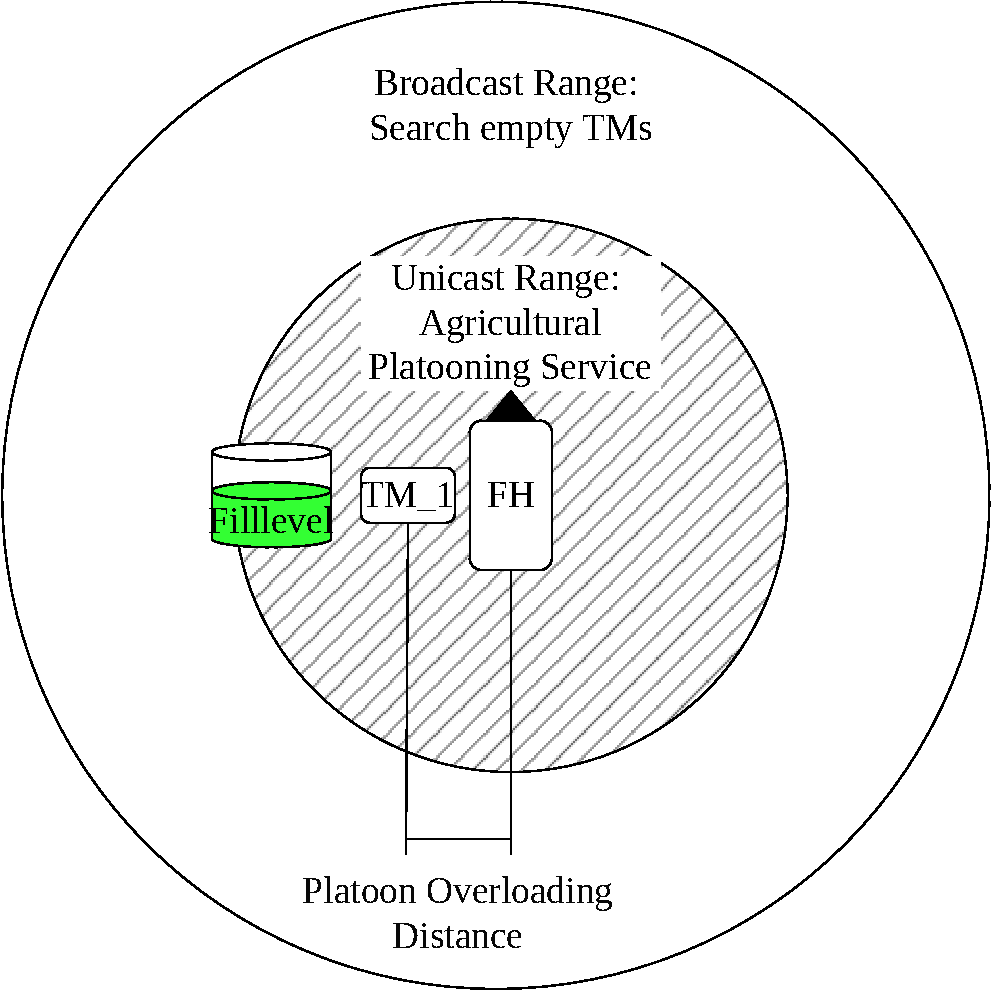
\includegraphics[width=0.6\textwidth]{figures/platoonHALF}
	\caption{\acf{TM} position left of the \acf{FH} for overloading, where the \ac{TM} is half full and the
		\ac{FH} starts \autoref{alg:SearchTM} to search for a next empty \ac{TM},
		which can later take over the loading position.}
	\label{fig:PlatooningHF}%
\end{figure}
If the \ac{TM} fill level is half full, the \ac{FH} starts \autoref{alg:SearchTM}
to search for a new \ac{TM} to load the corn onto.
This process is visualized in \autoref{fig:PlatooningHF}.
As soon as the \ac{FH} finds a new \ac{TM}, the \ac{FH} connects to the new \ac{TM} and starts sending
the \ac{TM} guidance positions, which place the \ac{TM} \SI{12}{\metre} behind the \ac{FH}.
The \ac{FH} continues harvesting until the \ac{TM} is fully loaded.
Meanwhile, the new \ac{TM} is waiting behind the \ac{FH} and can take over the loading position next to the \ac{FH} as
soon as the \ac{TM}, where the \ac{FH} is currently loading onto, is full.

\begin{figure}[]%
	\centering
	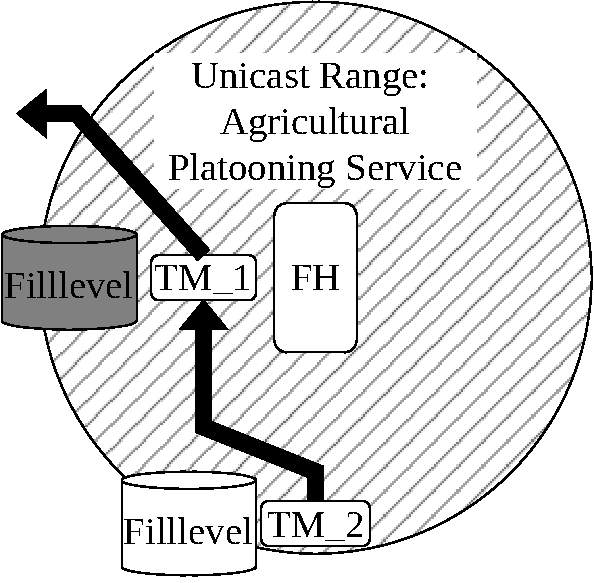
\includegraphics[width=0.33\textwidth]{figures/platoonFULL}
	\caption{Change of \acf{TM}s in the Application Agricultural Platooning Service, where $TM\_1$
	is full and leaves the field while the empty $TM\_2$ takes over the overloading position.}
	\label{fig:PlatooningFull}%
\end{figure}

A fully loaded \ac{TM} leaves the field to unload the corn and returns to the position where it disconnected from the \ac{FH}.
There, it waits for an incoming $search\_TM$ request from a \ac{FH} to connect to a \ac{FH} again.

The corn harvest process is finished when the last \ac{FH} has finished harvesting and moved to the end of the field as
shown in \autoref{fig:PlatooningRoute}.

\begin{table}[H]
	\centering
	\begin{tabular}{p{5cm}p{4cm}}
		\toprule
		Parameters & \\
		\midrule
		\textit{search\_TM\_interval} & \SI{1}{\second}\\
		\textit{search\_TM\_packet\_length} & \SI{0.5}{\kilo\byte}\\
		\textit{platoon\_data\_interval} & \SI{50}{\milli\second}\\
		\textit{platoon\_data\_packet\_length} & \SI{1}{\kilo\byte}\\
		Platoon Overloading Distance & \SI{5}{\meter}\\
		\ac{FH} Working Width & \SI{6.2}{\meter}\\
		\ac{TM} Volume & \SI{50}{\cubic\meter}\\
		\bottomrule
	\end{tabular}
	\caption{Simulation parameters for the Application Agricultural Platooning Service}
	\label{tab:SimulationParameters}
\end{table}

\subsubsection*{Simulation Verification}
Each corn harvest scenario is visualized to ensure the correctness of the simulation.
The visualizations are created with the ns-3 extension Netsimulyzer.
The corn field is marked as a black rectangle. Next to the lower left corner there is a cuboid which marks the location of the silo.
Every node was displayed as the Netsimulyzer model of a landdrone, where all \ac{FH}s are black and the
\ac{TM}s are either red, green, yellow or blue, depending on the \ac{TM} state.
\begin{figure}[H]%
	\centering
	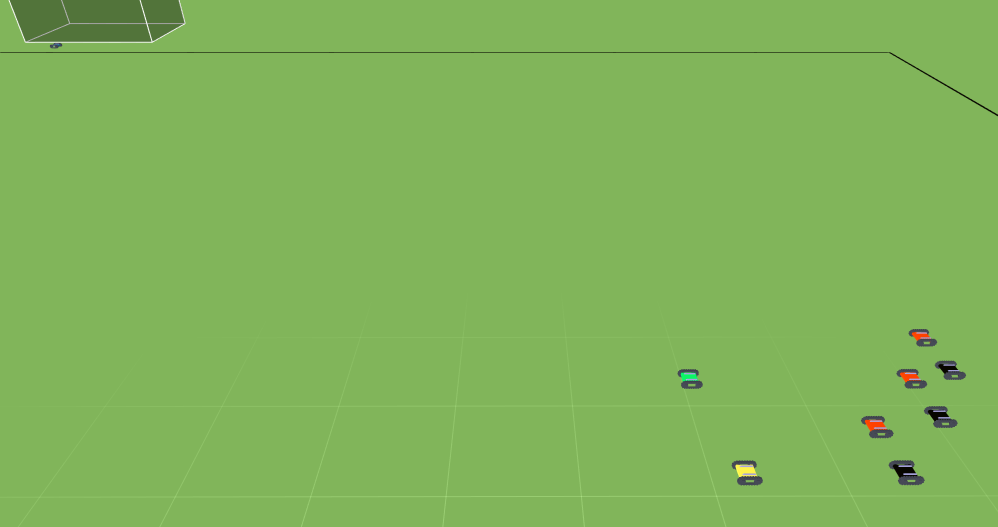
\includegraphics[width=0.75\textwidth]{figures/platooningScreen}
	\caption{Screenshot of the simulation visualization in Netsimulyzer, where a blue \acf{TM} is unloading in the back in front of the farm cuboid,
		two red \acp{TM} are in a Agricultural Platooning Service with the black \acf{FH}s,
		a green \ac{TM} is empty and waiting for a new $search\_TM$ request and a yellow \ac{TM} is in waiting position behind a black \ac{FH}.}
	\label{fig:PlatooningScreenshot}%
\end{figure}

An empty \ac{TM} is displayed green and changes to yellow as soon as it is associated with a \ac{FH} and in waiting position behind the \ac{FH}.
The \ac{TM} is red as soon as the \ac{FH} starts loading the corn onto the \ac{TM} in an Agricultural Platooning Service.
A full \ac{TM} is displayed blue and moves to the farm cuboid next to the lower left corner of the field.
As soon as the \ac{TM} is empty, it changes back to green and waits for a new \ac{FH} to connect to it at the last disconnection position.

I use this visualization to verify the correct mobility of the \ac{FH} and the \ac{TM}, the correct \ac{TM} state transitions,
that the simulation is ending properly and that the \ac{FH} switches the waiting \ac{TM} after disconnecting
from the fully loaded \ac{TM}.

Using the provided information from the ns-3 MonitorSnifferRxCallback and MonitorSnifferTxCallback I was able to review ongoing transmissions and
whether the specified physical layer parameters are used correctly for non-uniform and uniform traffic.

Every simulation runs \num{2} \ac{TM}s per \ac{FH}.
This does not correspond to the key figures of 10 \ac{TM}s per \ac{FH} in the corn harvest scenario \cite{faustzahlen2018},
but is sufficient as there is no communication of \ac{TM}s while transporting the harvested crop to the farm currently planned.
For this reason, I have set the simulation so that a full \ac{TM} is empty again after \SI{10}{\second} at the disconnect position.
This is a reasonable value, as it ensures that every time a \ac{FH} starts a $search\_TM$ request, there is a \ac{TM} in range to connect to.

\textcite{zhang_method_2009} defined a data frame of \SI{32}{\byte}, which includes an identifier, timestamp, longitude,
latitude, heading, speed and direction.
This set of data comprises a basic set which is sufficient for the implementation of a platooning service,
as the authors show.
\textcite{schlingmann_aef_2019} do not specify the amount of data further and point out that the required data rate
for platooning services is low.

The use case requirements for vehicle platooning services in \cite{TR-22.886} specify data sizes of \SIrange{300}{1200}{\kilo\byte},
depending on the vehicle density.

I have set the data size \textit{platoon\_data\_packet\_length} to \SI{1}{\kilo\byte} for the simulation of platooning services.
This data size is an abstraction of the storage space that may be needed for additional data or implementations
of authentication and security mechanisms.
In the Corn Harvest scenario, additional data could be, for example, the fill level of the transport machine,
information about the environment, obstacles or other machines on the field.

\textcite{zhang_method_2009} already showed that an interval of \SI{100}{\milli\second} is sufficient for Agricultural Platooning Services
in a harvest scenario.

I chose a $platoon\_data\_interval$ of \SI{50}{\milli\second} for the Agricultural Platooning Service
as \textcite{smolnik_5g_2020} mention that their requirements analysis indicated that new guidance data should at least arrive every \SI{50}{\milli\second}.

\section{Application Level Simulation Evaluation}
I chose the following simulation configurations for the uniform transmission of guidance data: \ac{HE}-\ac{MCS} 3, 5 and 7 and
\ac{STBC} either enabled or disabled.
Every simulation configuration runs \num{5} times, where every \ac{FH} harvests \SI{1}{\hectare} of corn, which equals to roughly
\num{2.5} \ac{TM} loads.
Every simulation run has a different random seed.
After the simulation run successfully and the simulation process is verified in the visualization,
a mean value and confidence interval with a confidence level of
\SI{95}{\percent} is calculated per simulation configuration.

The results for defined metrics latency and data update rate are shown in \autoref{fig:mean_50}.


\begin{figure}[]%
	\centering
	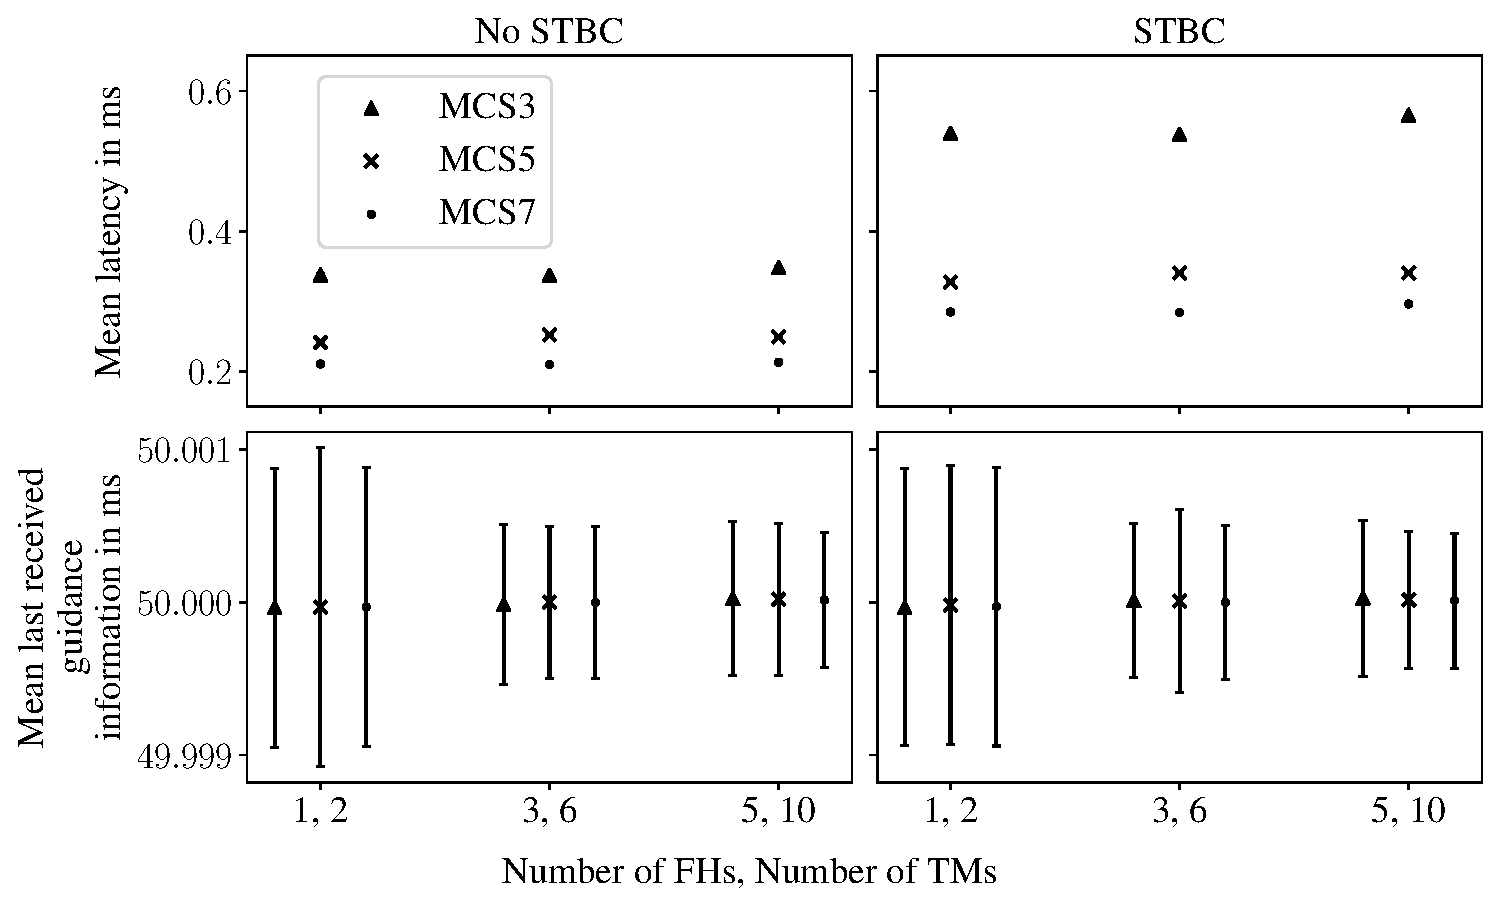
\includegraphics[width=0.95\textwidth]{figures/latency_lastUpdate50ms}
	\caption{Mean latency and mean guidance data update interval of the Application Agricultural Platooning Service in regards to the number of \ac{FH}s and \ac{TM}s and
	the chosen \ac{HE}-\ac{MCS} value for a $platoon\_data\_interval$ of \SI{50}{\milli\second}.}
	\label{fig:mean_50}%
\end{figure}

The desired $platoon\_data\_interval$ of \SI{50}{\milli\second} can be achieved with every
configuration.

The confidence interval for the mean update rate is always below \SI{2}{\micro\second}.
The mean latency is always below \SI{0.6}{\milli\second}.
Using higher \ac{HE}-\ac{MCS} values reduces the mean latency of
the Agricultural Platooning Service data exchange.

Applying \ac{STBC} additionally increases the mean latency compared to
non- \ac{STBC} configurations.
This is due to the fact that the \ac{STBC} configuration uses the redundant copy of data to
improve the reliability of the transmission by applying maximum likelihood decoding.
This decreases the data rate and increases
the mean latency.
Nevertheless, the desired $platoon\_data\_interval$ of \SI{50}{\milli\second} can be achieved when using \ac{STBC} for
every specified \ac{HE}-\ac{MCS} value and thereby increase the reliability of the transmission.

The recorded process data from the corn harvest scenario showed that the \ac{FH} can also harvest at higher speeds around
\SI{10}{\kilo\meter\per\hour} than can be calculated from the key figures in \cite{faustzahlen2018}.
To test the applicability of the Agricultural Platooning Service for higher speeds, I ran a additional simulation where I changed the
harvest states according to \autoref{tab:harvestStatesChanged}.

\begin{table}[H]
	\centering
	\begin{tabular}{>{\centering}p{2cm}p{4cm}p{4cm}}
		\toprule
		Harvest State & \ac{PD} & \ac{FH} speed\\
		\midrule
		H0 & \SI{20}{\tonne\per\hectare}
        & \SI{14}{\kilo\metre\per\hour} (\SI{3.89}{\metre\per\second}) \\
		H1 & \SI{30}{\tonne\per\hectare}
        & \SI{12}{\kilo\metre\per\hour} (\SI{3.33}{\metre\per\second}) \\
		H2 & \SI{50}{\tonne\per\hectare}
        & \SI{10}{\kilo\metre\per\hour} (\SI{2.78}{\metre\per\second}) \\
		\bottomrule
	\end{tabular}
	\caption{Corn harvest states, which define a range of \acf{PD}s from \cite{faustzahlen2018} and \acf{FH} speeds, which I set higher than the key figures in \cite{faustzahlen2018} specify to
	increase the requirements on the Agricultural Platooning Service.}
	\label{tab:harvestStatesChanged}
\end{table}

As I increased the \ac{FH} speed, which leads each harvest platoon, the whole platoon harvests the field faster.
Therefore, all \ac{TM}s move faster.
To provide faster \ac{TM}s more often with guidance data,
I decreased the $platoon\_data\_interval$ to \SI{25}{\milli\second} to ensure,
that a \ac{TM} always stays in the harvest platoon position even at higher speeds.

This $platoon\_data\_interval$ of \SI{25}{\milli\second} heads in the direction of the upper required update rate of \SIrange{10}{25}{\milli\second} for general
vehicle platooning services in \cite{TR-22.886}.
But the values in \cite{TR-22.886} correspond to higher platoon sizes, a velocity of \SI{100}{\kilo\meter\per\hour} and a
vehicle distance of \SIrange{1}{2}{\metre}.


\begin{figure}[]%
   \centering
   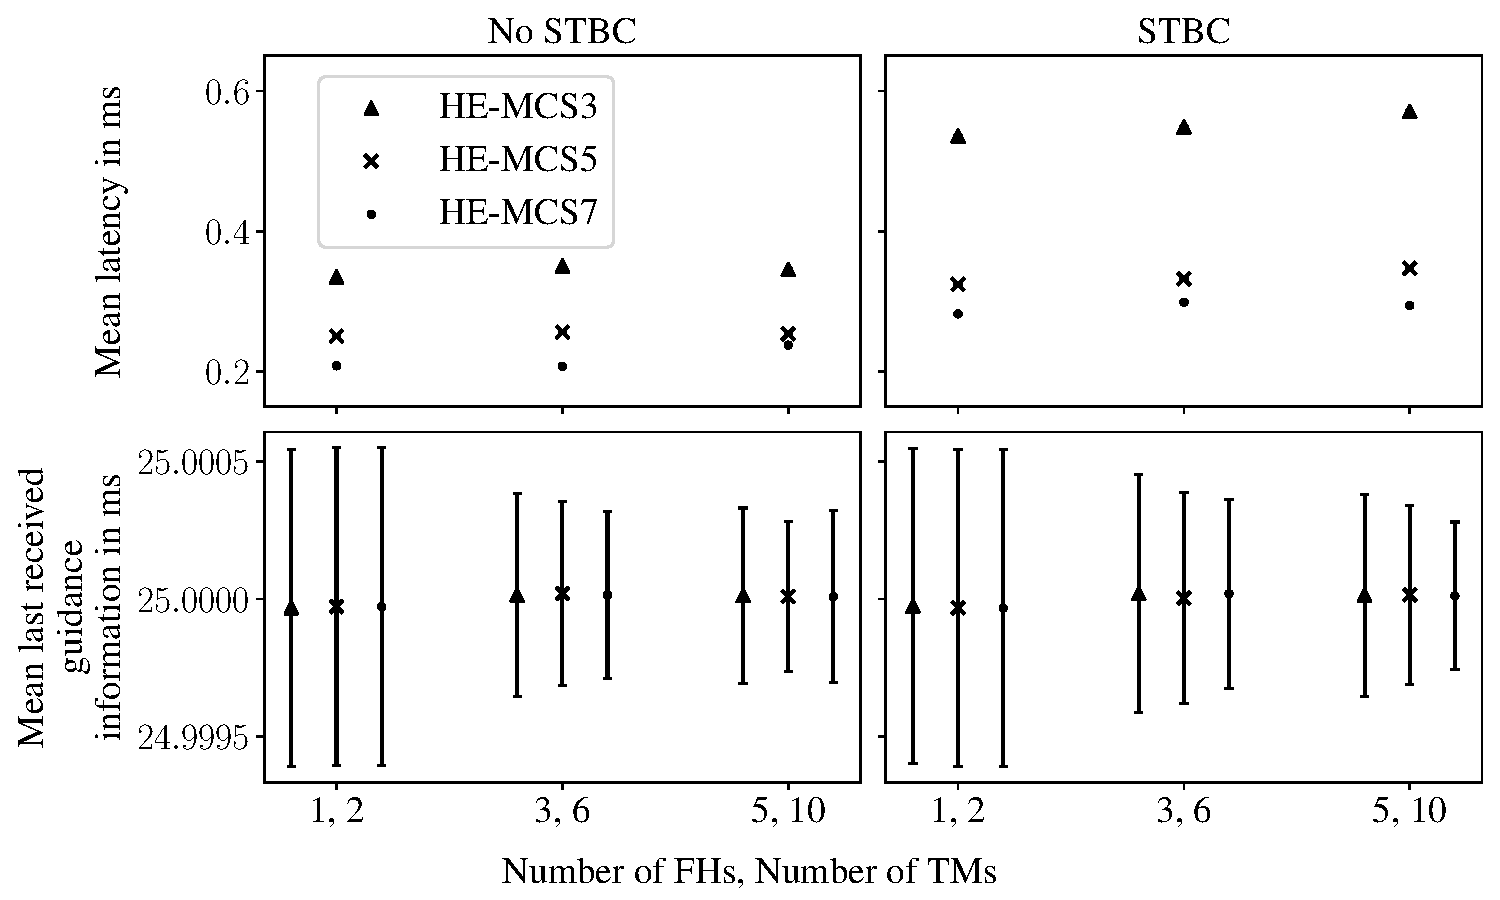
\includegraphics[width=0.95\textwidth]{figures/latency_lastUpdate25ms}
   \caption{Mean latency and mean guidance data update interval of the Application Agricultural Platooning Service in regards to the number of \ac{FH}s and \ac{TM}s and
   the chosen \ac{HE}-\ac{MCS} value for a $platoon\_data\_interval$ of \SI{25}{\milli\second}.}
   \label{fig:mean_25}%
\end{figure}

The simulation runs with the same physical layer configurations as in \autoref{fig:mean_50}.
The results displayed in \autoref{fig:mean_25} reveal that the mean guidance data update interval is always around \SI{25}{\milli\second},
which is the desired $platoon\_data\_interval$.
The mean latency is nearly the same as in \autoref{fig:mean_50}, which indicates that there is still some channel capacity left for
further data exchange.

Both simulations were based on the abstracted and simplified corn harvest scenario, which is based on the ns-3 communication model and
abstracted implementation of the physical layer and MAC layer in ns-3.
In a real-world scenario, an Agricultural Platooning Service has to operate in the complex agricultural environment, which
may impact signal propagation and communication performance.

The simulated communication is based on a \ac{BW} of \SI{20}{\mega\hertz}, which offers the highest possible signal power spectral density.
Additional robustness is gained by using \ac{STBC}, \ac{LDPC}, low \ac{MCS} values and \ac{CR}s which are encoded for example in
\ac{HE}-\ac{MCS}3 and are available since the IEEE 802.11n standard.
These physical layer configurations are enough to transmit guidance data in an Agricultural Platooning Service.

Both simulations did not consider the impact of interference due to other ongoing transmissions.
For example, \ac{WIC} Video streaming services can increase the network load and consequently lead in higher latencies for
the Agricultural Platooning Service.
A solution would be to prioritize the Agricultural Platooning Service over other services
to ensure a certain quality of service.
When passing houses, industrial, or farm buildings, additional Wi-Fi transmissions can be expected.
Interference with other Wi-Fi
transmissions can easily occur, when the channel is heavily loaded.
The results showed that some channel capacity is still left for further data exchange of other channel users.
Since a narrow bandwidth of \SI{20}{\mega\hertz} is used, interference is less likely compared to wider bandwidths,
as a wider spectrum is likely to be more utilized if transmission in the frequency spectrum are equally distributed.


Using IEEE 802.11ax, a new service discovery transmission mode is available.
Additionally, to the lowest \ac{MCS} and \ac{CR},
IEEE 802.11ax can apply the \ac{ER} mode with \ac{DCM} which increases robustness as shown in \autoref{sec:Robustness}
and therefore increases the communication range.
This physical layer amendment is designed to introduce a new level of long-range communication in IEEE 802.11.
At the moment, I am not aware of any research that measured the resulting communication range in an agricultural environment.

If the communication range is not sufficient for service discovery, a road side unit at the field entrance can be used to exchange \ac{FH} position data
between \acp{TM} leaving and entering the field.
Alternatively, a field planner can be used to give an overview of where a \ac{FH} should be harvesting,
when everything works as expected.
These two options can provide \ac{FH} position estimations, which can be used to guide \acp{TM} to a position where they are likely
to receive service discovery broadcasts from \acp{FH}.







